%%%%%%%%%%%%%%%%%%%%%%%%%%%%%%%%%%%%%%%%%
% Masters/Doctoral Thesis 
% LaTeX Template
% Version 2.5 (27/8/17)
%
% This template was downloaded from:
% http://www.LaTeXTemplates.com
%
% Version 2.x major modifications by:
% Vel (vel@latextemplates.com)
%
% This template is based on a template by:
% Steve Gunn (http://users.ecs.soton.ac.uk/srg/softwaretools/document/templates/)
% Sunil Patel (http://www.sunilpatel.co.uk/thesis-template/)
%
% Template license:
% CC BY-NC-SA 3.0 (http://creativecommons.org/licenses/by-nc-sa/3.0/)
%
%%%%%%%%%%%%%%%%%%%%%%%%%%%%%%%%%%%%%%%%%

%----------------------------------------------------------------------------------------
%	PACKAGES AND OTHER DOCUMENT CONFIGURATIONS
%----------------------------------------------------------------------------------------

\documentclass[
12pt, % The default document font size, options: 10pt, 11pt, 12pt
oneside, % Two side (alternating margins) for binding by default, uncomment to switch to one side
english, % ngerman for German
onehalfspacing, % Single line spacing, alternatives: onehalfspacing or doublespacing
%draft, % Uncomment to enable draft mode (no pictures, no links, overfull hboxes indicated)
%nolistspacing, % If the document is onehalfspacing or doublespacing, uncomment this to set spacing in lists to single
%liststotoc, % Uncomment to add the list of figures/tables/etc to the table of contents
%toctotoc, % Uncomment to add the main table of contents to the table of contents
%parskip, % Uncomment to add space between paragraphs
%nohyperref, % Uncomment to not load the hyperref package
headsepline, % Uncomment to get a line under the header
%chapterinoneline, % Uncomment to place the chapter title next to the number on one line
%consistentlayout, % Uncomment to change the layout of the declaration, abstract and acknowledgements pages to match the default layout
]{MastersDoctoralThesis} % The class file specifying the document structure

\usepackage[utf8]{inputenc} % Required for inputting international characters
\usepackage[T1]{fontenc} % Output font encoding for international characters
\usepackage{todonotes}
\usepackage{mathpazo} % Use the Palatino font by default

%\usepackage[style=numeric]{biblatex} % Use the bibtex backend with the authoryear citation style (which resembles APA)
\usepackage[backend=bibtex,style=numeric]{biblatex}
\bibliography{main} 

\usepackage[autostyle=true]{csquotes} % Required to generate language-dependent quotes in the bibliography

%----------------------------------------------------------------------------------------
%	MARGIN SETTINGS
%----------------------------------------------------------------------------------------

\geometry{
	paper=a4paper, % Change to letterpaper for US letter
	inner=2.5cm, % Inner margin
	outer=3.8cm, % Outer margin
	bindingoffset=.5cm, % Binding offset
	top=1.5cm, % Top margin
	bottom=1.5cm, % Bottom margin
	%showframe, % Uncomment to show how the type block is set on the page
}

%----------------------------------------------------------------------------------------
%	THESIS INFORMATION
%----------------------------------------------------------------------------------------

\thesistitle{Developing Automatic Network Testing for an Ad-hoc Heterogeneous Mesh Network} % Your thesis title, this is used in the title and abstract, print it elsewhere with \ttitle
\supervisor{Dr. Paul \textsc{Gardner-Stephen} \linebreak Dr. Saeed \linebreak \textsc{Rehman}} % Your supervisor's name, this is used in the title page, print it elsewhere with \supname
\examiner{} % Your examiner's name, this is not currently used anywhere in the template, print it elsewhere with \examname
\degree{Bachelor of Engineering(Software)(Honours)} % Your degree name, this is used in the title page and abstract, print it elsewhere with \degreename
\author{Lachlan Brock} % Your name, this is used in the title page and abstract, print it elsewhere with \authorname
\addresses{} % Your address, this is not currently used anywhere in the template, print it elsewhere with \addressname

\subject{Software Engineering} % Your subject area, this is not currently used anywhere in the template, print it elsewhere with \subjectname
\keywords{} % Keywords for your thesis, this is not currently used anywhere in the template, print it elsewhere with \keywordnames
\university{\href{https://www.flinders.edu.au/}{Flinders University}} % Your university's name and URL, this is used in the title page and abstract, print it elsewhere with \univname
\department{\href{https://www.flinders.edu.au/college-science-engineering}{College of Science and Engineering}} % Your department's name and URL, this is used in the title page and abstract, print it elsewhere with \deptname
\group{The Douglas Adams Institute For Implausible Linguistics} % Your research group's name and URL, this is used in the title page, print it elsewhere with \groupname
\faculty{\href{}{}} % Your faculty's name and URL, this is used in the title page and abstract, print it elsewhere with \facname

\AtBeginDocument{
\hypersetup{pdftitle=\ttitle} % Set the PDF's title to your title
\hypersetup{pdfauthor=\authorname} % Set the PDF's author to your name
\hypersetup{pdfkeywords=\keywordnames} % Set the PDF's keywords to your keywords
}

\begin{document}

\frontmatter % Use roman page numbering style (i, ii, iii, iv...) for the pre-content pages

\pagestyle{plain} % Default to the plain heading style until the thesis style is called for the body content

%----------------------------------------------------------------------------------------
%	TITLE PAGE
%----------------------------------------------------------------------------------------

\begin{titlepage}
\begin{center}

\vspace*{.06\textheight}
{\scshape\LARGE \univname\par}\vspace{1.5cm} % University name
\textsc{\Large Honours Thesis}\\[0.5cm] % Thesis type

\HRule \\[0.4cm] % Horizontal line
{\huge \bfseries \ttitle\par}\vspace{0.4cm} % Thesis title
\HRule \\[1.5cm] % Horizontal line
 
\begin{minipage}[t]{0.4\textwidth}
\begin{flushleft} \large
\emph{Author:}\\
{\authorname} % Author name - remove the \href bracket to remove the link
\end{flushleft}
\end{minipage}
\begin{minipage}[t]{0.4\textwidth}
\begin{flushright} \large
\emph{Supervisors:} \\
{\supname} % Supervisor name - remove the \href bracket to remove the link  
\end{flushright}
\end{minipage}\\[3cm]
 
\vfill

\large \textit{A thesis submitted in fulfilment of the requirements\\ for the degree of \degreename}\\[0.3cm] % University requirement text
%%\groupname\\\deptname\\[2cm] % Research group name and department name
 
\vfill

{\large \today}\\[4cm] % Date
%\includegraphics{Logo} % University/department logo - uncomment to place it
 
\vfill
\end{center}
\end{titlepage}

%----------------------------------------------------------------------------------------
%	DECLARATION PAGE
%----------------------------------------------------------------------------------------

\begin{declaration}
\addchaptertocentry{\authorshipname} % Add the declaration to the table of contents
\noindent I, \authorname, declare that this thesis titled, \enquote{\ttitle} and the work presented in it are my own. I confirm that:

\begin{itemize} 
\item This work was done wholly while in candidature for a degree of \degreename.
\item This document is in accordance with the plagiarism policy of \univname.
\item Where any part of this thesis has previously been submitted for a degree or any other qualification at this University or any other institution, this has been clearly stated.
\item Where I have consulted the published work of others, this is always clearly attributed.
\item Where I have quoted from the work of others, the source is always given. With the exception of such quotations, this thesis is entirely my own work.
\item I have acknowledged all main sources of help.
\item Where the thesis is based on work done by myself jointly with others, I have made clear exactly what was done by others and what I have contributed myself.\\
\end{itemize}
 
\noindent Signed:\\
\rule[0.5em]{25em}{0.5pt} % This prints a line for the signature
 
\noindent Date:\\
\rule[0.5em]{25em}{0.5pt} % This prints a line to write the date
\end{declaration}

\cleardoublepage

%----------------------------------------------------------------------------------------
%	QUOTATION PAGE
%----------------------------------------------------------------------------------------

\vspace*{0.2\textheight}

\noindent\enquote{\itshape Add quotation later}\bigbreak

\hfill Add who I attribute it to

%----------------------------------------------------------------------------------------
%	ABSTRACT PAGE
%----------------------------------------------------------------------------------------

\begin{abstract}
  \addchaptertocentry{\abstractname} % Add the abstract to the table of contents

  This is a brief overview of the whole thesis, andis between 200-300 words. It should specify precisely and succinctly what the thesis is about. It should be written in such a way as to attract the reader's interest. The abstract should answer three questions: What? Why? How?

\end{abstract}

%----------------------------------------------------------------------------------------
%	ACKNOWLEDGEMENTS
%----------------------------------------------------------------------------------------

\begin{acknowledgements}
\addchaptertocentry{\acknowledgementname} % Add the acknowledgements to the table of contents
But most of all I thank me for writing this (add later)
\end{acknowledgements}

%----------------------------------------------------------------------------------------
%	LIST OF CONTENTS/FIGURES/TABLES PAGES
%----------------------------------------------------------------------------------------

\tableofcontents % Prints the main table of contents

\listoffigures % Prints the list of figures

%\listoftables % Prints the list of tables

%----------------------------------------------------------------------------------------
%	ABBREVIATIONS
%----------------------------------------------------------------------------------------

%\begin{abbreviations}{ll} % Include a list of abbreviations (a table of two columns)

%\textbf{LAH} & \textbf{L}ist \textbf{A}bbreviations \textbf{H}ere\\
%\textbf{WSF} & \textbf{W}hat (it) \textbf{S}tands \textbf{F}or\\

%\end{abbreviations}

%----------------------------------------------------------------------------------------
%	PHYSICAL CONSTANTS/OTHER DEFINITIONS
%----------------------------------------------------------------------------------------

%\begin{constants}{lr@{${}={}$}l} % The list of physical constants is a three column table

% The \SI{}{} command is provided by the siunitx package, see its documentation for instructions on how to use it

%Speed of Light & $c_{0}$ & \SI{2.99792458e8}{\meter\per\second} (exact)\\
%Constant Name & $Symbol$ & $Constant Value$ with units\\

%\end{constants}

%----------------------------------------------------------------------------------------
%	SYMBOLS
%----------------------------------------------------------------------------------------

%\begin{symbols}{lll} % Include a list of Symbols (a three column table)

%$a$ & distance & \si{\meter} \\
%$P$ & power & \si{\watt} (\si{\joule\per\second}) \\
%Symbol & Name & Unit \\

%\addlinespace % Gap to separate the Roman symbols from the Greek

%$\omega$ & angular frequency & \si{\radian} \\

%\end{symbols}

%----------------------------------------------------------------------------------------
%	DEDICATION
%----------------------------------------------------------------------------------------

%\dedicatory{For/Dedicated to/To my\ldots} 

%----------------------------------------------------------------------------------------
%	THESIS CONTENT - CHAPTERS
%----------------------------------------------------------------------------------------

\mainmatter % Begin numeric (1,2,3...) page numbering

\pagestyle{thesis} % Return the page headers back to the "thesis" style

% Include the chapters of the thesis as separate files from the Chapters folder
% Uncomment the lines as you write the chapters

% Chapter Template

\chapter{Introduction}\label{chapter:firstchapter} % Main chapter title

\label{Chapter1} % Change X to a consecutive number; for referencing this chapter elsewhere, use \ref{ChapterX}

\section{Communication without infrastructure}
When a disaster strikes, communication often goes with it.
Communication is crucial in modern life — doubly so when a disaster leaves people in danger.
Unfortunately, when a disaster strikes a region, communications are often some of the most vulnerable infrastructure.
Even if the disaster does not directly affect communications infrastructure, this infrastructure is often overwhelmed by victims attempting to contact rescue teams.
\todo{Rewrite, this is all weak}
This impact is  further compounded in areas with already insufficient communication infrastructure such as remote areas and poorer regions.
Because of this, there is significant demand for cheap, reliable, and resilient communications methods for remote and disaster-affected regions.
Developed in response to the 2010 Haitian earthquakes that led to the loss of over 100,000 lives and crippled communication infrastructure, severely hampering rescue efforts, the Serval Project aims to provide emergency communications in disaster struck areas through the deployment of the Serval Mesh Extenders.

\section{The Serval Mesh Network}
\todo{Add intro bit}
To achieve communication without pre-existing infrastructure, the Serval team developed the Rhizome protocol.
Rhizome is a store-and-forward protocol, with every Rhizome node having its own database that stores all files when it receives them, and forwards files to any neighbouring nodes that require them.
The end result of this is that Serval networks are able to guarantee that every file is received by its destination node, however it does not guarantee the time that this will take.
The Rhizome protocol was initially implemented as an ad hoc WiFi only mesh network that could be used in a disaster zone to allow communication without infrastructure.
Today, the Serval Mesh now supports WiFi, UHF packet radio, and an experimental HF radio implementation, with more radio communication methods being developed.
To handle these various communication methods, the Serval Mesh consists of two main software components; Servald and LBARD.
Servald in the main implementation of the Rhizome protocol, and handles the core functionality of Serval devices, from adding to the Rhizome database to handling the encryption of messages for transfer, and also supports synchronisation with other nearby Serval devices over WiFi.
LBARD stands for Low Bandwidth Asynchronous Rhizome Demonstrator, and serves to facilitate sending and receiving Rhizome bundles over low bandwidth links such as UHF radio.

As it stands, the Serval Mesh network has several issues.
The first of these issues are several long-standing bugs in LBARD and the protocols it uses to synchronise messages with other LBARD nodes.
Further, due to the nature of Serval networks, it is difficult to set up real Serval networks to easily test the functionality of the network.
\todo{Change this structure around}

To assist with this, the Serval team have developed a software emulation framework to emulate the functionality of real Serval devices and networks.
While this has proven valuable with diagnosing issues with Serval functionality, the framework tests tend to test only the core Servald and LBARD functionality, without a focus on proper network functionality.
\todo{Add more about limitations}

\section{Problem Statement}
This thesis focuses on the development of additional testing tools for the Serval network, and the analysis of how these tools assist the Serval team with the development of the Serval Mesh.

To structure the development of this thesis, four research questions were developed.
These questions were:
\begin{enumerate}
    \item \firstRQ
    \item \secondRQ
    \item \thirdRQ
    \item \fourthRQ
\end{enumerate}
Each of these four questions is answered in depth throughout this thesis.


\section{Structure of this thesis}

This thesis will focus on the three main contributions made to the Serval project through this Honours project.
The first of these is the comprehensive overview and identification of the limitations in LBARD and the Serval test framework as outlined in Chapter 3.

The next contribution is the improvement of the test framework, and the development of several diagnostic and visualisation tools to assist with the analysis of both emulated and real-world tests which is detailed in Chapters 4, 6, and 6. 
In Chapter 7, these developed tools are thoroughly discussed, with the strengths and limitations of these critically analysed, and their contribution to the goals of the Serval project verified. 
\todo{Verified is not the right word}

The third main contribution is outlined in Chapter 7, and involves the use of the developed tools to identify significant faults in LBARD, as well as verifying the correction of these faults.
These developed tools also used to determine the simulation fidelity — that is, how accurate the test framework is to real-world scenarios.
\todo{Fix this, not actually the case anymore}

Finally, in Chapter 8 the main results of this thesis are summarised, and the future work outlined.
\todo{Add more/fix}


% Chapter Template

\chapter{Literature Review} % Main chapter title

\label{Chapter2} % Change X to a consecutive number; for referencing this chapter elsewhere, use \ref{ChapterX}

%----------------------------------------------------------------------------------------
%	SECTION 1
%----------------------------------------------------------------------------------------

\section{Mesh Networks}
A Mesh Network is a type of wireless network where each device directly connects to any neighbouring devices within range.
To communicate over longer distances than a single device can communicate, each device in the network - called a node - act as a relay, where they transmit any data they receive to their neighbouring nodes.


\begin{itemize}
    \item What they are
    \item How they work
    \item What the advantages are
    \item What the different types are (partially connected/fully connected)
\end{itemize}

\section{The Serval Mesh Network}
\begin{itemize}
    \item What is Serval?
    \item How does it work (Servald, LBARD, bundles, pieces, etc.)
    \item Different radio types
    \item Last bit is LBARD
    \item What are we doing (testing network)?
\end{itemize}

    
\subsection{The Serval Project}
In 2010, Dr. Paul Gardner-Stephen began the development of the Serval Mesh Network in response to the earthquakes in Haiti. 
Originally, the network was designed to connect smartphone devices together using WiFi and Bluetooth technology to form an ad hoc mesh network.
However, through development this was abandoned due to the lack of ad hoc WiFi support in Android and iOS devices.
To circumvent this, the first generation Serval Mesh Extender was developed.
This Mesh Extender was built using a GL-AR150 portable WiFi router, and was able to reach ranges of up to 100 meters.
With this Mesh Extender, users could connect their smartphone devices to the wireless hotspot of the Mesh Extender without requiring their smartphones themselves to become a node in the mesh network.
To extend the range of these Mesh Extenders further than the 802.11 WiFi would allow, a radio module was added to the Mesh Extender.
The RFD900 radio module allowed for Serval Mesh Extenders to reach ranges of up to 3 kilometres over the 915MHz radio band.

\todo{Talk about 2nd gen mesh extenders}


\begin{itemize}
    \item The history
    \item Original mesh plan — smart phones over wifi
    \item 1st gen mesh extenders
    \item 2nd gen mesh extenders
    \item Tested in field in Vanuatu
\end{itemize}


\subsection{Rhizome}
The Rhizome protocol was developed for the Serval Mesh Network, and forms the basis of all services provided by the Serval Mesh.

Rhizome has several features that are useful for the Serval Mesh network.
The first of these is that it functions as a store and forward protocol, where when data is transferred across the mesh network, this data is stored on the Serval node that this data is transferred to, and is then forwarded on to any neighbouring nodes that do not have this piece of data.
In practice, this means that the Serval Mesh is very rugged, as the data sent through the Mesh will be stored in multiple locations so that even if one node is removed from the network due to a situation such as a natural disaster or power outage, then this data will still — eventually — reach its destination as long as a path can be made to the destination.
The other advantage that the store-and-forward design has is that the Mesh does not need to use any routing protocols to determine what the most efficient route to the destination is; the data will eventually reach every node and will naturally find the most efficient route to the destination.

Further, the decentralised nature of Rhizome means that there is no central point of failure or central location where the networks data is stored; it is stored on every node.
This is vitally important in situations such as disaster recovery where the Serval Mesh will be used in areas where it is possible that a Rhizome node may be lost.

Rhizome uses two data structures, a manifest and a payload.
A Rhizome payload is simply a unit of data such as an image file, or a message.
A manifest lists all meta-data associated with this payload, including the size, data type, date of creation, and intended destination.
A Rhizome Bundle is formed of a manifest and a payload. 

\todo{Benefits}

\subsection{Serval-DNA}
Serval-DNA forms the main software component of the Serval Mesh Network.
Written in C, Serval-DNA handles all the core functionality of the Serval Network and provides the implementation of the Rhizome protocol.

Serval-DNA handles the transfer of Rhizome Bundles over WiFi automatically, determining what bundles are required by nearby nodes through a synchronisation method.

\todo{Talk more about what/how it does}

\begin{itemize}
    \item What servald is
    \item How it works
    \item Overview of functionality
    \item Bundles/pieces/etc
\end{itemize}


\subsection{LBARD}
The Low Bandwidth Asynchronous Rhizome Demonstrator (LBARD) is a C program written for the Serval Project that handles synchronising Rhizome Bundles over low bandwidth connections such as those used in the RFD900 packet radio in the Serval Mesh Extender.
LBARD was developed to run as an addition to Serval-DNA and provides the functionality to communicate with neighbouring Serval nodes as well as implementing the radio drivers necessary to use the various radio types that LBARD supports.

Since the default synchronisation method for Rhizome as implemented in Serval-DNA relies on a relatively high amount of bandwidth in comparison with the low bandwidth available on UHF or HF radios a new synchronisation method needed to be used for these low bandwidth links.
LBARD uses a tree-synchronisation protocol that uses a XOR of Rhizome bundle hashes to quickly determine which bundles are missing from its neighbours. \todo{cite}
This synchronisation protocol allows for LBARD nodes to efficiently determine if a neighbour is missing any of the bundles that it has in its Rhizome store with a minimal amount of communication needed.
This is crucial for the low-bandwidth links that exist between two LBARD nodes, as it allows for LBARD to utilise the rest of the bandwidth that is available to it to transfer the Rhizome bundles. \todo{fix}
After the LBARD node has determined what bundles are required to be transferred, these bundles are then transferred in 64-byte pieces.
To ensure that these pieces are received, LBARD continues sending these pieces until it receives a confirmation from the receiving node that all the pieces have been received intact.

As it stands, LBARD is able to support several radio types, including the RFD900, with some experimental implementations for the CodanHF and BarrettHF radios, as well as a prototype Outernet satellite uplink.


\subsection{Serval Test Framework}
The Serval Test Framework is a test suite designed for the Serval Network, that provides the framework for emulated Serval nodes to be tested.
The test framework is largely written as Bash scripts that setup specified tests, and links Serval nodes together using simulated WiFi or radio connections.
The test framework is divided into two parts; the Serval-DNA framework, and the LBARD framework.
The framework provides the tools to test a wide range of Serval functionality, as it is able to directly monitor the performance and responses of the software and compare it to the expected output as defined in the test definition.
The framework functions as an emulator rather than a simulator as it is running the real Serval-DNA/LBARD software, with only the links between nodes simulated.
The Serval Test Framework will be covered in more detail in Chapter 3.

\subsection{Serval Test Network}
\begin{itemize}
    \item Talk briefly
    \item What it is, observers, etc.
\end{itemize}

\section{Network Testing}

\begin{itemize}
    \item More general; what are methods to network testing?
    \item Simulation?
    \item Emulation? Difference?
    \item Real world/bench testing?
    \item Large-scale real-world tests
    \item How it's done
    \item Why it is important
    \item What are important features
    \item Why we don't want to use 
    \item What improvements Serval needs
\end{itemize}

\subsection{Features of Popular Test Frameworks}


\subsection{Network and Graph Visualisation}
\begin{itemize}
    \item What emulators had graphical outputs
    \item What visualisation is helpful
    \item What tools exist \& what offers the best fit
\end{itemize}


\section{Summary}
\begin{itemize}
    \item In comparison with other networks
    \item 
\end{itemize}
 
\chapter{Description and analysis of existing test framework} 
\label{Chapter3} 

In a project like the Serval project, confidence in its performance is crucial — particularly if it will be used in disaster recovery efforts.
To achieve this, both the development team and potential users of the network need to be confident in its performance in a wide range of scenarios. 
While a significant portion of this will need to be done through field testing, this is unfeasible to perform without software emulation.

The test frameworks for Serval-DNA and LBARD were developed to perform software testing by emulating the real Serval software and analysing its behaviour during tests.
In this chapter, the first research question "\firstRQ" will continue to be answered as was started in Chapter 2. 


\section{Aims of test frameworks}
The Serval-DNA test framework was built to test the functionality of the Serval mesh in its early days when nodes were purely communicating over WiFi. 
This emulator is able to emulate multiple aspects of the Serval DNA software, from validating the database integrity to simulating WiFi communication between Serval nodes. 
Later, once LBARD was added to the Serval project, a second emulator was built that extended the code of the Serval DNA emulator.
This emulator performed similar functions to that of the Serval DNA emulator; testing internal LBARD functionality, and emulating radio communication between Serval nodes. 
While the LBARD emulator serves as an extension to the Serval DNA emulator — extending and overwriting functionality — there is currently no ability to run tests that feature both WiFi and radio links. 


\section{Serval DNA Test Framework}
The Serval DNA test framework is a bash script that serves as the basis of Serval testing with over 200 tests written.
These tests are also bash scripts that import the necessary functions from the framework. 
The test framework provides functions for setting up and running tests, as well as handling functionality such as starting and stopping \texttt{servald} instances.
With this framework, these test scripts are able to model a wide range of Serval functionality, allowing for developers to easily and effectively write tests with a minimal amount of boilerplate code required \parencite{servalTestDocumentation}.

The test framework is composed of three major parts; the test framework, the test definitions, and the test file.
The framework (\texttt{testframework.sh}) provides the functions necessary to run tests, including: command line argument parsing, running tests, stopping tests, and monitoring log files. 

The test definitions file (\texttt{testdefs.sh}) provides specific functions that are needed for specific test files.
These functions include setting up, configuring and starting Serval instances.
When running specific types of tests, the \texttt{testdefs.sh} file can be extended by other files such as in the case of the \texttt{testdefs\_rhizome.sh} file. 
This allows for some functions provided in the testdefs file to be overwritten, allowing for different functionality depending on the type of test; this is used when attempting to use different configurations than that provided by the original \texttt{testdefs.sh} file.

Finally, the test files themselves are where tests are defined. 
These files import the test definitions and test framework and define the environment and test conditions necessary to run tests. 
Running the tests requires running the appropriate test file and the framework and definitions will be imported automatically.

\section{LBARD Test Framework}
The LBARD test framework extends the functionality of the Serval DNA test framework, however it overrides multiple functions to get it working with LBARD.
By overriding functions, the LBARD test framework is able to create Serval instances running LBARD and is able to simulate radio links between these nodes between the \texttt{fakeradio} program.
\texttt{Fakeradio} monitors the driver outputs of each LBARD network interface, and routes these packets to the simulated driver inputs of the appropriate LBARD interfaces according to the rules specified in the test definition.
Network topologies can be specified with \texttt{fakeradio} by defining the radio links allowed between LBARD nodes.

When a test is run, the test framework starts the specified number of Serval instances, each with their own separate databases, configurations, and log files.
LBARD instances are then started for each of these instances, running emulated radio hardware (RFD900, BarrettHF, etc.) as defined in the test definition.
Finally, Fakeradio is started and begins to listen to the output files of each of the LBARD interfaces.
Once a test is concluded, the framework collects all the log files and outputs of the Serval instances, LBARD instances, and Fakeradio.
These are then collated into a single test log file, with every piece of data timestamped.

\emph{Unless otherwise specified, when talking about the test framework in this document, we will be talking about the LBARD test framework.}


\subsection{Defining Tests}
Tests are defined in either the lbard (\texttt{./lbard/tests/lbard}) or lbard\_size\_tests (\texttt{./lbard/tests/lbard\_size\_tests}) file. 
These are Bash files that import the LBARD test framework, and define what tests are to be run.
Tests are comprised of three basic components: a doc string with a brief description of what the test does, a \texttt{setup} function that sets up the test environment, and a \texttt{test} function, that is run when the test is run.
The doc string is used when running tests and serves as feedback to the tester as to what test is currently being run.
The \texttt{setup} function is run before the test is conducted. 
This function serves to set up any necessary configurations for the running of this test such as \texttt{fakeradio} rules, or adding files to Serval instances.

Finally, in the test function, the conditions for a successful test are defined. Once this function completes (or an error/fail/timeout is encountered), the test concludes.


This can be seen in Figure \ref{fig:testDefinition}. 
In this figure, the \texttt{setup} function defines the Fakeradio rules, then adds a single file of 50 bytes to the Serval instance A. 
In the test function, a function \texttt{all\_bundles\_received} is defined, that simply checks if instance B received a bundle with the specified bundle ID and version. 
The test then waits until this bundle is received. 
If this bundle is received before the default timeout, the test will pass.

\lstset{language=bash,
showstringspaces=false,
numbers=left,
}

\begin{figure}
    \begin{centering}

\begin{lstlisting}[breaklines, frame=single]
doc_OneOne="FAKE RADIO (RFD900) - A single very small bundle transfers to a single peer"
setup_OneOne() {
    lbardparams="allow between 0,1; deny all;"
    setup 0 0 0 "\${lbardparams}" 
    # Insert a file to server A
    set_instance +A
    rhizome_add_file file1 50
}
test_OneOne() {
    # Test that the bundle arrives at server B
    all_bundles_received() {
        bundle_received_by $BID:$VERSION +B 
    }
    wait_until all_bundles_received
} 
\end{lstlisting}
        \caption{Example of LBARD test definition}
        \label{fig:testDefinition}
    \end{centering}
\end{figure}

\subsection{Existing Tests}
Currently, 276 LBARD tests exist; 55 of these are in \texttt{./tests/lbard} file, and 221 of these are in the \texttt{./tests/lbard\_size\_tests} file.

Of these, only 14 of these tests are unique, with all the tests in the \texttt{lbard\_size\_tests} following the same format with the only difference in the size of the bundle increasing in increments of 10 bytes from 6000 to 8200 bytes.

The majority of the tests in the LBARD test file are as follows, with slight difference in test variables:
\begin{itemize}
    \item Detect radio types (RFD900, BarrettHF, CodanHF)
    \item Setup for Outernet
    \item Outernet up-link tests with various sizes
    \item One peer to one peer with BarrettHF
    \item One peer to one peer with various sizes
    \item MeshMS with different packet loss
    \item File delivery with 3 hops over UHF (RFD900)
    \item 10 nodes sending, 10 receiving, various LBARD options
    \item 10 nodes sending, 10 receiving, various packet sizes
\end{itemize}


\section{Outputs}
Tests produce two main outputs; a PASS/FAIL status in the command line, and a log file.
As shown in \figurename{ \ref{fig:exampleTest}} when a test is run, four possible status messages can be displayed; pass, fail, error, and fatal.
\begin{list}{}{}
    \item \texttt{PASS} occurs when a test has fulfilled the requirements outlined in the test definition.

    \item \texttt{FAIL} occurs when a test does not meet the requirements from a test definition but it is not due to an issue with the test or test definition. This may occur if a timeout elapses, or an output does not meet a success condition.
    
    \item The \texttt{ERROR} status occurs when an error occurs that stops the test from running correctly, such as LBARD failing to start properly, or being failing to start Serval DNA with the current configuration.
    
    \item Finally, the \texttt{FATAL} status occurs when files are missing, commands are not available, or invalid options are passed to the test framework.
\end{list}

\begin{figure}
    \begin{centering}
        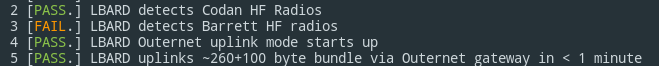
\includegraphics[width=14cm,height=20cm,keepaspectratio]{Figures/testOutput1.png}
        \caption{Example output of LBARD tests}
        \label{fig:exampleTest}
    \end{centering}
\end{figure}

The produced log file contains the outputs of all the programs run in the course of the test including \texttt{servald} and \texttt{LBARD} instances, \texttt{fakeradio}, and the test framework, with each line in the log file timestamped.
The log files produced contain several pieces of information.
At the beginning of the file the name, status, and start/finish time of the test is listed.
Next, the complete logs of each of the started sub-processes are listed.
Tests can be configured to display more log information by setting specific flags in the configuration of the test.


\section{Limitations}
While the emulators are able to test large portions of the Serval network, they have several limitations that drastically limit the usefulness of the emulators to effectively model real world situations.
The first limitation is that it is currently not possible to model networks that use WiFi alongside radio, limiting the testable scenarios to that of just WiFi if using the Serval-DNA framework, or just radio networks if using the LBARD framework.

Another major limitation of the test frameworks is that there currently exists very few topologies that are being tested.
While the Serval DNA portion of the framework does feature various WiFi-exclusive topology tests including long node chains and a 6 node circular network these are minimal,
and the LBARD framework only features topologies of chain networks
Due to the previous limitation, this means there are no currently existing topology tests that contain multiple radio types or WiFi/radio networks.

While the log files produced by the tests are extensive and contain a large amount of data that is helpful while debugging, it does have several drawbacks.
Firstly, with just the log files and the status message it is difficult to determine where errors are occurring in a test, particularly in initial stages of debugging network topologies.
Partially, this is due to the log files not being chronologically ordered, but instead ordered by what log file it is, and \emph{then} chronologically ordered.
This means that attempting to work out where an error occurred becomes a process of consistently switching places in the large log file.
When more detail has been located about the issue — such as which device it occurred on, then it is useful to go through the large log file.

The log file has a further limitation, as the partially chronological ordered log has no information about network topology or graphical output, hindering efforts to explain network issues.

Finally, as topology tests have not been extensively tested, it is difficult to determine the simulation fidelity.
Without a comparison between the test framework and real-world scenarios, the simulation fidelity is impossible to determine. 
This can lead to a lack of confidence in the results of the emulated tests, and may lead to issues occurring in the real-world that do not occur in the emulation.


\section{Suggested Improvements}
To improve the LBARD test framework, multiple changes will need to be made.
The first of these is adding the ability to allows nodes to communicate over both WiFi and Fakeradio.
This step alone will drastically increase the scope of possible tests that can be conducted, as it will allow for tests of both WiFi and emulated Fakeradio interface.
Further, this will allow for networks to utilise more than one type of radio communication.

With the ability to have multiple link types between Serval nodes, a much larger range of network topologies can be modelled and tested.
Adding more network topologies to the test framework will allow for a much more detailed testing, and will almost certainly uncover previously undiscovered issues with the Serval network as it has simply not been possible to test complicated network topologies in emulation before.

To allow testers to more effectively debug the results of a test, a simpler log file will need to be generated.
This log file should contain only the crucial log information from a test, and the log lines should be formatted in a consistent format and chronologically ordered.

To improve on the ability to understand and communicate the functionality of specific Serval network topologies, some form of graphical output will need to be created, allowing for testers to see the network undergoing testing, as well as the data moving around the network.
This will almost certainly prove beneficial to the Serval team on two fronts. 
Firstly, this will assist Serval developers in isolating and locating bugs in Serval networks by visually showing them the functioning of a network, supplementing the expansive log files that the frameworks produce.
Further, this will assist Serval team members communicating where issues are occurring as the diagrams can act as a supplement to the explanation.

Finally, once the emulator can model a variety of network topologies, the simulation fidelity of the emulator should be determined.
To achieve this, the emulator should model a real-world Serval network and run tests on this network, and then those same tests should be run on a real-world implementation of this network.
This will serve to validate the accuracy of the Serval emulator, as it is expected that modelling the same network should have near-identical results with minimal variance provided the appropriate variables (i.e. average packet loss) have been accounted for in the emulation.

\section{Summary}
In this chapter the first research question "\firstRQ" and the third research question "\thirdRQ" have both been answered.
To analyse the state of the test framework, its aims first needed to be analysed. 
This aim of the Serval-DNA framework was determined to be: provide the basis for validating the functionality of core Serval functionality.
The aim for the LBARD framework was determined to be: provide the basis for field tests, and validate LBARD functionality, particularly the tree-synchronisation and the radio drivers.

In this chapter, both the Serval-DNA and LBARD test framework were analysed in detail, and an explanation and outline provided of their core functionality.
The process for defining tests and a detailed analysis of the two main output types of the frameworks was conducted.
The limitations of the frameworks was outlined, and then a list of recommendations of improvements that should be made to the test frameworks was listed, answering the third research question.
In the next chapter, the first of these improvements will start to be implemented, beginning the answering of the fourth research question "\fourthRQ.
The improvements that will be implemented is adding the functionality to allow WiFi to run alongside radio in a test and then more topology-focused tests will be added to the framework.
% Chapter Template

\chapter{Extending the Test Framework} % Main chapter title
\label{Chapter4}

%----------------------------------------------------------------------------------------
%	SECTION 1
%----------------------------------------------------------------------------------------

\begin{itemize}
    \item Modify test framework
    \item Modify fakeradio to output layout
    \item Get dual link types working
    \item Be able to define different WiFi layouts
    \item 
\end{itemize}


\begin{itemize}
    \item Currently, no way to easily determine what topology is in machine readable format
    \item What info is needed for this 
    \item How can we represent it?
    \item Why format?
    \item JSON vs CSV
\end{itemize}


%-----------------------------------
%   SECTION 1
%-----------------------------------
\section{Joint WiFi \& Radio Tests}
A key part of the test framework that was missing was support for networks with both WiFi and radio link types. 
This presents a major limitation  to the test framework as real Serval networks would feature both of these network links.
To implement this feature, several additions need to be made to the test framework.

First, the ability to define which link simulation will be used for each nodes needs to be defined.
This allows test definition writers to define the functionality(??) of each of the nodes. 
For instance, test writers are able to define if a specific node in a topology is using the fakeradio tool or simply acting as WiFi, or even, both. 

Next, the ability to define specific network topologies will need to be added.
This already exists in the case of the fakeradio networks as discussed in the previous chapters, this is not easily done with the simulated WiFi tool.

Once these two pieces of functionality have been added to the test framework, developers will be able to test considerably larger and more complicated network topologies with ease.
With this expanded test framework the Serval team will be able to significantly improve their knowledge of the Serval network; complicated, larger, and reproducible tests offer a huge benefit to the goals of the Serval team. \todo{rewrite, this is bad}

What needed to be done for this?
\begin{itemize}
    \item Add capability to define interface to use
    \item Strip definitions to get lists of what interfaces for each node
    \item For each node, add the interfaces that are in lists
    \item For each node, add appropriate configuration
    \item Pass LBARD rules to fakeradio as per normal
\end{itemize}

\todo{Mention that this is done in a NEW FILE}
\todo{Add new testdefs file}

To achieve this, several features need to be implemented. 
The first feature is defining the interfaces to be used on a per-node basis.
With this, nodes can each have their own configuration, allowing for some nodes to have WiFi enabled while others only have fakeradio interfaces.
Next, the ability to define WiFi topologies will need to be added, as currently it appears to only be possible to have nodes communicating with every other node without any defined topology.

To ensure that this does not affect pre-existing LBARD tests, two new files will be created.
The first is the \verb|topologies| test file.
This file is just a new test file that outlines the new tests to be implemented.
Further, since these will need 

\subsection{Defining interfaces per node}
\begin{itemize}
    \item \textbf{Explain original scenario}
    \item Pass n nodes, all are labelled as specified radio type
    \item n Serval interfaces and n LBARD interfaces are started
    \item fakeradio is started
    \item Test is run, communicate, log it all
    \item Limitation: as it is treating each node the same with no differentiation between, no way to enable wifi on some nodes and not others
\end{itemize}
\todo{briefly explain original scenario}

\todo{Explain why we need to enable interfaces}

The first step to completing this is to determine what nodes need which configuration applied.
Two possibilities exist for this; manually define the configurations for each node or automatically determine which configuration is required for each node.
Since each node that will be connected by fakeradio needs to be defined already, it was decided to use this information to determine what configuration the node needed.

Each test that uses fakeradio contains a string in the setup function defining the links between nodes.
An example of this is shown in \todo{add figure}. 
The string defines the links in the format "allow between [n],[m];" where n and m are the 0-indexed serval-dna instance number.
This is suitable to use since every node in a topology using fakeradio must be specified in this string, meaning that \verb|every| node that requires LBARD interfaces defined will be listed here.
As the WiFi functionality does not need to have the topology defined in such a way it is necessary to define a new string, simply listing the nodes that require WiFi to be enabled. 

These strings are passed to the \verb|start\_instances| function. 
To determine what nodes to enable the configurations on, the node information needs to be stripped from the string.

To achieve this, multiple alterations need to be run on the strings.
The first is removing newline characters and replacing them with spaces.
This ensures that multiple line fakeradio rules will not break the node parsing.
Next, a \verb|sed| command is run, replacing every character that is not a number with a space character, stripping all information that is not specifically the number of the node.
The \verb|tr| command is then run, removing extraneous space characters, so that the string is just the node numbers separated by a single space character.
Finally, each space character is replaced with the \verb|sed| command with a newline character.
This results in two string of the node numbers, with each node on a new line.
To use these in the rest of the program, these strings are converted to an array, one for WiFi and one for fakeradio nodes.

With this information, we can now programmatically determine which configurations need to be enabled on each nodes.
To implement this however, one more step is required.
A new array \verb|all\_nodes| is created that simply lists all of the nodes in the test.
This array simply contains the combined unique set of the WiFi and fakeradio arrays.

Next, the program iterates through the \verb|all\_nodes| array, and adds the string 'wifi', 'fakeradio' or 'wifi fakeradio' to an array of strings at the index of the node.
This results in an array where at the index of a given node the interfaces are textually listed.
\todo{add better explanation - diagram?}
The framework then iterates through each node specified and sends the array to the \verb|configure\_servald\_server| function.


The \verb|configure\_servald\_server| is called for each node before the instance is started, and as such each configuration is unique to each instance of servald.
This means that we can now add the required configuration for a node without affecting other nodes.
When the configure\_servald\_server function is called the program simply calls the \verb|add\_servald\_interface| function with the interfaces needed for that given node.
When this is called the program iterates through the supplied interfaces (ie. 'wifi', 'fakeradio', or 'fakeradio wifi') and for each interface configures the servald instance appropriately.
For fakeradio instances, the only configuration that needs to be set is enabling http (to connect to LBARD) and setting the username and password for LBARD.

With this completed, it is now possible to run WiFi and fakeradio nodes side-by-side, with the appropriate interfaces enabled based on the test definition.
However this method has a major limitation; it is not possible to have complicated WiFi topologies with this method since WiFi nodes have zero restriction around what other WiFi nodes they can communicate with.
This means that while networks such as \todo{figure a; A-r-B-w-C-r-D} work, any network such as \todo{figure b} will not work as there is no way to restrict node E from connecting to node C.



\subsection{Defining wifi topologies}
When expanding the test framework to handle the mixed topologies, it was planned to implement functionality to define WiFi network layouts in the same format as defining fakeradio networks, however it was suggested to instead define wifi interfaces using existing tools found in the Serval-DNA framework.
While this meant that topology tests would be not have a consistent method of defining network layouts between radio and WiFi nodes, it would however be consistent with Serval-DNA tests.

Using the method previously outlined in the previous section, WiFi nodes all default to using the same WiFi interface - thus creating a fully-connected WiFi mesh sub-network, leading to every WiFi node being connected. 
This can be seen in \figurename{ \ref{fig:networkWifi1}}.
Each WiFi interface is essentially a sub-network, with nodes within a specified interface only able to communicate with nodes within the same interface as themselves.
Thus, to define a complicated network topology it is necessary to restrict which interfaces WiFi nodes can communicate on.

\begin{figure}
    \begin{centering}
        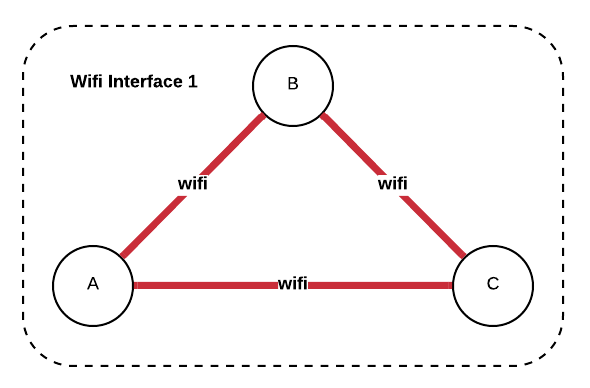
\includegraphics[width=14cm,height=20cm,keepaspectratio]{Figures/networkWifiInterface1.png}
        \caption{Network topology without defining interfaces}
        \label{fig:networkWifi1}
    \end{centering}
\end{figure}


In the Serval-DNA test framework, non- fully-connected WiFi networks are created by manually defining the WiFi interfaces that a specified servald interface is connected to.
To implement this, several changes need to be made.
The first is removing the functions added in the previous section that relate to WiFi.
This is because we'll no longer be defining WiFi nodes with a string passed to the setup functions.
Next, it was decided for every node to automatically have WiFi functionality enabled by default, but only connected to its own private interface. 
This is done by changing the configuration parsing added in the previous section to enable WiFi by default, but still only enabling LBARD as specified.

To connect nodes via WiFi they must now be connected to a specific WiFi interface as shown in \figurename{ \ref{fig:definingInterfaces}}.

\begin{figure}
    \begin{centering}
        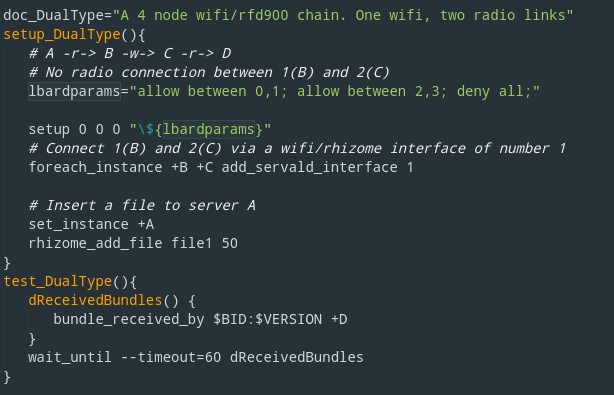
\includegraphics[width=14cm,height=20cm,keepaspectratio]{Figures/definingInterfaces.png}
        \caption{Defining WiFi interfaces}
        \label{fig:definingInterfaces}
    \end{centering}
\end{figure}
When a node is connected to multiple nodes at once, it will be able to communicate with all other nodes in those interfaces, while the connected nodes are still only able to communicate with nodes in the same interfaces as themselves.
This means that previously impossible network topologies such as WiFi chains can be implemented as shown in \figurename{ \ref{fig:networkWifi2}}.

\begin{figure}
    \begin{centering}
        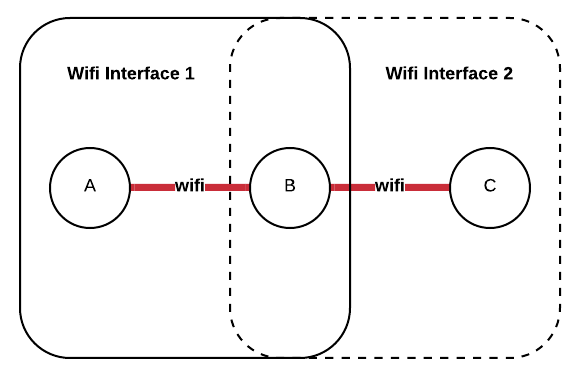
\includegraphics[width=14cm,height=20cm,keepaspectratio]{Figures/networkWifiInterface2.png}
        \caption{Network topology with two wifi interfaces defined}
        \label{fig:networkWifi2}
    \end{centering}
\end{figure}


\section{Adding utility functions}
\begin{itemize}
    \item Add ability to define {n} things
    \item Add ability to define multiple radio types easily
\end{itemize}


\section{Adding more topologies tests}
\begin{itemize}
    \item List the ones that existed previously - only used for development
    \item We need more than just the basic ones defined earlier
    \item Not just wifi/radio
    \item Complicated topologies (find some that represent real models and reference)
\end{itemize}

\section{Summary}
\textbf{Add link to next section. "While these improved things, we still need to add more. So graphical output blah blah"} 
\chapter{Improving the Output} % Main chapter title

\label{Chapter5} % Change X to a consecutive number; for referencing this chapter elsewhere, use \ref{ChapterX}

\lstset{language={},
showstringspaces=false,
numbers=none,
}

%----------------------------------------------------------------------------------------
%	SECTION 1
%----------------------------------------------------------------------------------------

In this chapter the fourth research question "\fourthRQ" will continue to be answered by developing a tool that allows for a simple log file to be and graphical representations of network traffic throughout a test to be generated.


\section{Creating a Simple Log}
As outlined in Chapter \ref{Chapter3}, the generation of a simple log file will allow for testers to more effectively test the Serval network by filtering out unnecessary log information and providing a consistent and chronologically ordered log file.

The log file generated by this tool will require six main features.
\begin{itemize}
    \item Consistent formatting
    \item Chronological ordering by timestamp
    \item Reduce amount of information to only useful info
    \item Machine \emph{and} human-readable layout information
    \item Log traceability to original log file
    \item Support all pre-existing topology tests
\end{itemize}

To generate this simple log file, there are three main options; modify Serval software to improve the logging, modify the test framework, or develop a new tool to generate a simpler log file from the output of the test framework.
Modifying the outputs of Serval software was not considered to be a useful use of this thesis, as this would require changing large parts of the codebase for these programs for a relatively mild improvement, as well as modifying the code of tested and running devices.

Modifying the test framework was considered, however while this does solve the issue of the previous proposed solution this would add a large amount of bloat to the test framework that is not required in the vast majority of the tests, and may actually prove to be either impossible or vastly difficult using the Shell scripts of the test framework.
Further, this will increase the run-time for tests unnecessarily.

The final option is to write a program that after a test is run and the log file produced, processes the log file and filters and simplifies it, and outputs a separate, simpler log file. 

Finally, the use of an external tool to generate the simple log files was considered.
This is the method that will be undertaken in this thesis. 
The program will be written in C as it needs to be fast, portable, and use minimal external dependencies. 
Further, it is the language that the majority of the Serval codebase is written in, allowing for future developers to easily maintain and improve the code.

The developed program follows a simple process as shown in \figurename{ \ref{fig:chapter5SimpleFlowchart}}.
For each line in the log file, two steps are followed.
First, the line is filtered to determine if it should appear in the simple log file. 
Then, for each line that passes through the filter, apply some transformations to it if necessary so it is in a more useful format.
Different transformations may be used for different types of lines in the log file.

\begin{figure}[h!]
    \begin{centering}
        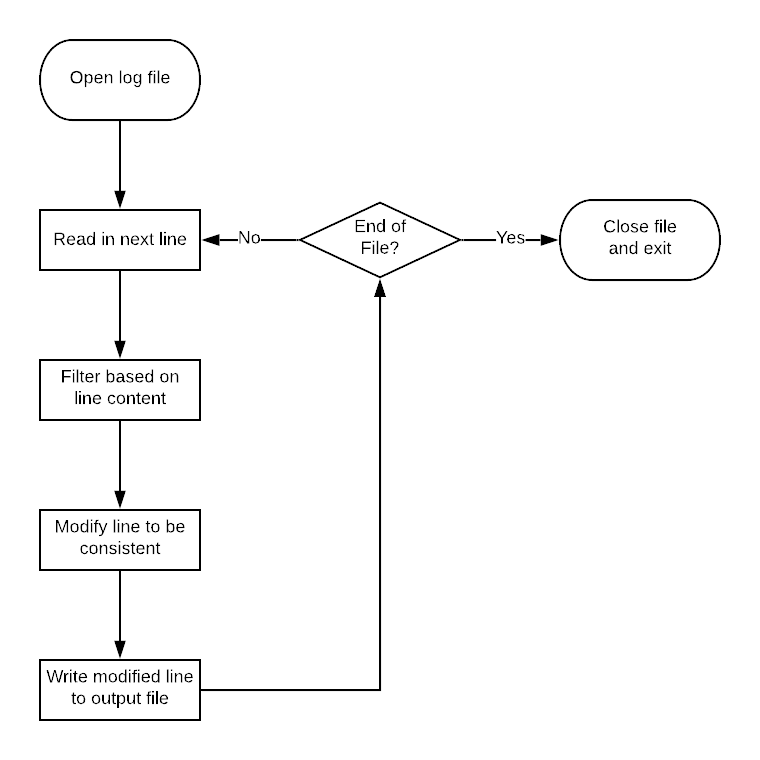
\includegraphics[width=10cm,height=20cm,keepaspectratio]{Figures/Chapter5-SimpleLogFlowchart.png}
        \caption{Flowchart of creating the simple log}
        \label{fig:chapter5SimpleFlowchart}
    \end{centering}
\end{figure}

\pagebreak
\subsection{Filtering Lines}\label{filteringLines}
To minimise the lines added to the simple log file, the initial input file needs to be filtered.
This allows for only specific lines to be added to the log file by adding only the lines which meet specific criteria. 

To determine the minimal information required to understand the tests, the output log files of the tests were analysed.
While analysing the output log files, the following list of important events was created.
\begin{itemize}
    \item \textbf{Setup} Start of a process, \texttt{LBARD}/Fakeradio
    \item \textbf{Setup} Test details
    \item \textbf{Setup} Layout information (WiFi and \texttt{fakeradio})
    \item \textbf{Setup} SID information
    \item \textbf{Servald} Sending and receiving packets
    \item \textbf{Servald} Adding manifest
    \item \textbf{LBARD} Neighbour has a bundle
    \item \textbf{LBARD} Send and receive bundles
    \item \textbf{Fakeradio} Any transfer between two nodes
\end{itemize}

This list covers all major aspects of a topology test; transfer of bundles, setup and layout information, sending and receiving general packets (including the tree-sync packets), and some internal logic and processing when packets are sent and received.
With only these important events, it should be possible to locate and isolate issues related to transferring bundles and packets. 
From there, these filtered events should allow a tester to more easily utilise the vastly more expansive and detailed original log file produced by the test framework. 

Once the desired events had been determined, these then needed to be filtered within the program.
To achieve this, each line in the file is analysed to determine if it is important by examining what substrings the line contains.
A line is accepted if it matches specified criteria; for instance, a line within the \texttt{fakeradio} process that contains the substring "\texttt{neighbour has a bundle}" would be considered important. 
These lines are then sent to the relevant function to be formatted appropriately.

\subsection{Output format}

\subsubsection{Formatting lines}
The log files produced by the test framework follow a consistent structure.
The structure always follows the structure of:
\begin{itemize}
    \item the test details, 
    \item the output of the test framework, 
    \item output of \texttt{fakeradio}, 
    \item output of \emph{each} \texttt{LBARD} process, and finally,
    \item the output of \emph{each} \texttt{servald} process.
\end{itemize} 

As this structure is consistent throughout tests in the framework, this allows the tools to only track which process is being processed, and then filter lines based on this.
However, the test framework log files have one major issue: the format of lines is not consistent between processes.
For instance, the typical \texttt{servald} line may appear as
\begin{center}
    \begin{lstlisting}[basicstyle=\small, breaklines]
DEBUG:[511710] 18:15:34.372 overlay_mdp.c:859:_overlay_send_frame() {mdprequests} Send frame 68 bytes    
    \end{lstlisting}
\end{center}
while a similar line in \texttt{LBARD} follows a format of:
\begin{center}
    \begin{lstlisting}[basicstyle=\small, breaklines]
T+25138ms : Sending length of bundle 6A1A3379501553D1* (bundle #0, version 1596098704035, cached_version 1596098704035)
    \end{lstlisting}
\end{center}

As shown above, the format between these two lines is clearly different and as such need to be formatted differently.
To achieve this, when a line is filtered as outlined in the previous section, the program returns an integer value representing the type of line that is to be formatted.
With this information, the appropriate formatting function can be called for the line type, so that it can be formatted correctly.

For \texttt{servald} lines this is trivial, the C standard function \texttt{sscanf} is used to extract the important information from the line and this information is then written to the simple log output file \texttt{sprintf}.

However, in the case of \texttt{LBARD} and \texttt{fakeradio} lines, multiple issues arise due to the formatting of the log files.
The first of these issues is that several lines in \texttt{LBARD} are not timestamped with the time that they occurred, rather they are timestamped with the number of milliseconds since the program started as shown above.
This is an issue since this means that the log files can not be easily sorted by timestamp, and also will not be formatted with a consistent format with the other lines.
To fix this, the initial time that an \texttt{LBARD} instance is started as logged by the file will be used as the T=0 point.
After this has occurred, when an event with a 'T+' timestamp is encountered, the number of milliseconds is added to the original timestamp to produce an accurate timestamp for this event.

The other issue with this method is that \texttt{fakeradio} log lines often are spread over multiple lines.
This means that simply scanning and processing a single line will not produce all the necessary information.
However, this can be mitigated by iterating over several lines until the end of this log line is reached.
As the program iterates through these lines it simply scans for the important information and forms a single log message from this.

With these outliers accounted for, the tool is now able to filter each log line in the initial log file and format these appropriately.


\subsubsection{Output log file}
With this, the log file produced now has a consistent format.
The simple log files format begins with the setup section.
The setup section lists all the essential information for drawing a diagram of the network topology. 
It lists the test details, SIDs of each of the nodes, and all the WiFi connections and \texttt{fakeradio} rules. 
An example of the setup section can be seen in \figurename{ \ref{fig:chapter5SimpleLogSetup}}.

\begin{figure}
    \begin{centering}
\begin{lstlisting}[frame=single]
#000 ====== BEGIN SETUP ======
#001 Name:     Wifi_RFD900_Chain_Short (topologies)
#002 Result:   PASS
#003 Started:  2020-08-24 13:22:55.044
#004 Finished: 2020-08-24 13:23:32.497
#005 SIDA : F170309E3033B957*
#006 SIDB : 86C9DD08EA6A4C65*
#007 SIDC : FA71E8E919914B52*
#008 SIDD : 41A35E8851578F82*
#009 SIDE : 954B6D94024986A0*
#010 SIDF : B38FB12CB39D006C*
#011 B connected to wifi interface 1
#012 C connected to wifi interface 1
#013 D connected to wifi interface 2
#014 E connected to wifi interface 2
#015 RULE: 'allow between 0,1'
#016 RULE: 'allow between 2,3'
#017 RULE: 'allow between 4,5'
#018 RULE: 'deny all'
#100 ======= END SETUP =======    
\end{lstlisting}
    \caption{Format of simple log setup}
    \label{fig:chapter5SimpleLogSetup}
    \end{centering}
\end{figure}

After the setup section, each line in the log file is ordered by chronological order. 
The lines follow a simple and consistent structure.
\begin{center}
    \begin{lstlisting}[basicstyle=\scriptsize, breaklines]
[Timestamp] [Process]:[Instance Letter] [Description]
    \end{lstlisting}
\end{center}

This structure can be seen in \figurename{ \ref{fig:chapter5SimpleLogFormat}}.
\begin{figure}
    \begin{centering}
\begin{lstlisting}[basicstyle=\small, breaklines, frame=single]
16:12:57.073 FAKERADIO A -> B [bundle piece]  bid=57E1F321* [229 bytes]
16:12:57.073 LBARD:A Broadcast tree sync message
16:12:57.091 LBARD:B Progress receiving 57E1F321*: Manifest is 258 bytes, and body is 50 bytes
16:12:57.091 LBARD:B We have the entire bundle 57E1F321*
16:12:57.092 SERVALD:B Adding 57E1F321F86F6197 to tree
16:12:57.092 SERVALD:B Queueing next message for 5ms   
\end{lstlisting}
        \caption{Format of simple log}
        \label{fig:chapter5SimpleLogFormat}
    \end{centering}
\end{figure}

\pagebreak
\section{Drawing Packet Transfer through the network}
To improve the output of the test framework, a network diagram displaying packet transfer is highly useful, allowing testers to better understand the topology they are testing. 
To produce a useful and informative network diagram, four steps need to be undertaken: determine the major events to be displayed on the diagram, create an ASCII representation of events during a test, generate a network diagram, and finally, create a PDF of the network topology with the traffic displayed.

\subsection{Getting Major and Minor events}
Before the network diagrams can be generated, the content that will be displayed must first be determined.
To do this, two categories of log events are defined: 
\begin{list}{}{}
    \item Major: When a node sends a message/packet to a node(s)
    \item Minor: Some processing on a single node that would not give the full picture of the test if omitted
\end{list}

Major events will be displayed in a diagram showing the network layout, showing the transfer between the two nodes and the message details. 
Minor events will be displayed in a list of minor events that occurred before the major event.
There can be multiple minor details per major event, however there is only one major event for each minor event.

There are two options for processing and sorting major and minor events.
The first is to process the simple log after it has been made, and check if a line should be considered major or minor. 
The other solution is to classify lines as they are processed in the creation of the simple log.
The second option is considerably faster, as in the first option we must re-process a new file and then classify lines within it to be major or minor, however the second option has a major issue in that when lines are classified during the creation of the simple log they are not yet sorted as the original log file is not sorted.
This means that if an array of major and minor events is created then these events will \emph{not} be in chronological order.
Unsorted events is an issue for the creation of diagrams as the created diagrams will then not be ordered.
This means that for the second option to be considered, a method of sorting and \emph{then} assigning minor events to a major event must be developed.
This is the approach that this thesis took.

Determining major events is simple; major events are a transfer between two nodes.
To save these major events, a struct defining major events is created.
This struct contains all the necessary features of a major event. These details are:
\begin{itemize}
    \item Sending Node
    \item All Destination Nodes
    \item Transfer details (type of message, size, etc.)
    \item The time it occurs at
    \item The transfer type (\texttt{LBARD} or WiFi)
    \item An array of minor events associated with this major event
\end{itemize}
Major events occur at two different points in the log file: when \texttt{fakeradio} sends a packet to a different node, and when \texttt{servald} sends a packet.
\texttt{Fakeradio} events are already filtered down to a one line log event for the simple log, so the program simply breaks this line down to get the details of the event, and then appends this to the major events array.
\texttt{Servald} events however, are more complicated as the packet transfer takes place over several messages.
To convert this into one event, the program saves the details of the packet as each line is processed until the log line stating that the message is sent, at which point all the saved details are added to an event and appended to the major event array.

To add the minor events, when a line for the simple log is being formatted for the simple log, the program simply checks if it meets a handful of criteria.
Since the log lines are just a single line, saving these minor events is as simple as appending these lines to the minor event array.


Once the simple log file has been produced, and all major and minor events have been extracted, each minor event needs to be associated with a major event.
When major and minor events are added to their respective arrays, they are done so in the order that the relevant lines appear in the input log file, meaning that these arrays are not chronologically sorted.
To associate a minor event with a major event, the minor event must occur before a major event, but \emph{after} the proceeding major event.
To achieve this, both of the arrays are sorted using the C standard function \texttt{qsort} with a comparator implemented that orders these by timestamp.

With the arrays sorted each minor array can be assigned to a major event.
This is done by assigning each minor event to a specific major event until this minor event occurs after the major event, at which point the next major event is chosen.
This iterates until every major event has had minor events assigned.
Any remaining minor events are assigned to a blank major event.

At this point, an array of all events throughout the test has been created with every minor event assigned to the appropriate major event.


\subsection{ASCII Network Traffic}
Creating an ASCII representation of the network traffic is trivial once minor and major events have been created.
To achieve this, the program simply iterates through every major event.
For each major event, the program then iterates through each minor event associated with this major event.
With this, the program is able to quickly print an ASCII representation of the network traffic through the network during a test.
This can be seen in \figurename{ \ref{fig:chapter5ASCIIRep}}.

\begin{figure}
    \begin{centering}
\begin{lstlisting}[numbers=left, basicstyle=\small, frame=single, breaklines, ]
38: [ 16:12:58.834] Tree sync message
    D -> BROADCAST
- 16:12:58.562 : LBARD:C We have new bundle 57E1F321*

39: [ 16:12:58.835 ] [LBARD instance identifier] [57 bytes]
    D -> C

40: [ 16:12:58.863] Tree sync message
    B -> BROADCAST
- 16:12:58.846 : LBARD:C Neighbour Node D (E31FC729) is missing bundle 57E1F321*
\end{lstlisting}
    \caption{ASCII Representation of test network}
    \label{fig:chapter5ASCIIRep}
    \end{centering}
\end{figure}
This output can then be piped to a file for debugging if testers do not have the requirements installed for generating the diagrams as outlined in the next sections.


\subsection{Generating a network diagram}
To render these diagrams, the network topology needs to be extracted from the test definition, then a diagram drawn of this topology.
From this layout, the image will then need to be created and rendered.
There are two main solutions for creating the image: do it using a graphics library, or creating a DOT file and rendering it with Graphviz.
Using a graphics library would provide a high level of control over the creation of the image as graphical elements would need to be defined explicitly and as such are unlikely to have unforeseen side effects as could be expected with using a higher-level solution such as Graphviz.
However, this would be considerably more complicated and harder to maintain than simply writing DOT files, then using the high-level tools provided by Graphviz to render this DOT file.
DOT files are text files that follow a specified syntax, and are used by Graphviz to render and create graphs.
These files are simple, and both human and machine-readable. 
It was decided that despite the far higher level of control possible by using a low-level graphics library, the accessibility, simplicity and maintainability of creating and rendering DOT files far outweighs this advantage.

To create this diagram, the topology information needs to be extracted from the test log.
For WiFi topologies, the test framework reports whenever a node is connected to a WiFi interface.
To create a diagram every time a node is connected to an interface, the interfaces that a specific node is connected to is saved in an array for each node.
To determine \texttt{fakeradio} topologies, when the \texttt{fakeradio} rules are reported in the log file, the links between nodes are extracted and this information added to a struct.
With this, the links between nodes have been determined, and a network diagram can be generated.

Once the simple log has finished being generated and the links between nodes gathered, the program then moves onto writing the layout DOT file.
The DOT file follows a simple format; initialisation of graph variables, and then the definition of the Layout sub-graph.
The graph is defined as a \emph{directed} graph.
This graph is defined as directed (but with arrow direction hidden) for the use in the network diagrams showing network traffic that will be discussed in the next section.

Producing the DOT file consists of four steps:
\begin{enumerate}
    \item Open the file and initialise variables
    \item Write the \texttt{fakeradio} links
    \item Write the WiFi nodes
    \item Write the end of the DOT file, then close it
\end{enumerate}

In the first step, the program opens a new file with the name \texttt{diagramLayout.dot}, and writes the initialisation variables.
The initialisation variables are the padding around the image the pen width to be used for drawing the diagram.

In the next step, the program simply iterates through each \texttt{fakeradio} link and defines a dashed link between these two nodes and colours it red.
This is used to highlight \texttt{fakeradio} links between nodes and help distinguish the different link types between nodes in a network.


Then, the program iterates through the WiFi link array. 
To do this, the program iterates through each of the interface arrays, and for each, defines a dashed link for all \emph{unique} combinations of the nodes in this interface which are then coloured blue.

Finally, the program adds the closing curly braces to the file, and closes it.
The program then renders the DOT file with the command:

\texttt{neato -Tpng [fileName] -o [outputFileName]}

An example DOT file and corresponding graph can be seen in \figurename{ \ref{fig:chapter5DotAndRender}}.
With this, the tool is able to create network topology diagrams using just the log information.
\begin{figure}[H]
    \begin{centering}
        \begin{minipage}{0.6\textwidth}
            \begin{lstlisting}[numbers=left, basicstyle=\small, breaklines, frame=l]
strict digraph A {
  ratio=fill
  pad=0.5
  mindist=0.5
  subgraph Layout {
    edge [dir=none, penwidth=3, style=dashed]
    A -> B [color=red]
    C -> D [color=red]
    B -> C [color=blue]
  }
}
            \end{lstlisting}
        \end{minipage}
        \begin{minipage}{0.15\textwidth}
            \raggedleft
            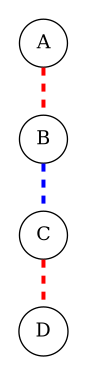
\includegraphics[height=9cm, keepaspectratio]{Figures/Chapter5-RenderedDot.png}
        \end{minipage}
        \caption{DOT file and rendered graph}
        \label{fig:chapter5DotAndRender}
    \end{centering}
\end{figure}

\subsection{Creating a LaTeX PDF}
To generate PDFs of the network traffic throughout the test, two steps must be made: create diagrams for each major event showing the network traffic during this major event, then add these diagrams and all minor events to a LaTeX template which is then rendered to a PDF.

\subsubsection{Transfer Diagrams}
The first step in creating a LaTeX PDF is to generate all the images of the network topology.
This is an extension of the development done in the previous section, however this is now creating multiple images — one per major event — and adding a directed link and label between a sending and receiving node.

To achieve this, the program iterates through every single major event and creates a new DOT file for each event.
In each file, the DOT file is created as previously outlined, however a new sub-graph is added named \emph{Transfer}
The transfer sub-graph contains a single solid line definition of a \emph{directed} connection between the sending and receiving node.
To display the transfer on this directed link between the nodes, a label is added that displays the transfer message.

With this, the DOT file can be compiled as previously described to generate a diagram for each major event.
When these are compiled in the LaTeX PDF, this will have the effect of appearing to animate the network topology.


\subsubsection{Creating the LaTeX PDF}
Once the diagrams have been created, a LaTeX PDF can then be created.
This PDF contains several pieces of information:
\begin{itemize}
    \item The test details
    \item A diagram for each major event
    \item All minor events associated with that major event
    \item The time the major event occurs
\end{itemize}
The produced LaTeX file follows a simple structure.
At the top of every page, the details of the test (name, result, and start/finish time) are listed.
Underneath this, the time that the major event occurred is listed. 
The vast majority of the page is taken up by the diagram of the network layout, showing the network traffic when the major event occurs.
Finally, the bottom half of the page is a list of minor events associated with the major event.

To produce this, the program follows a simple process.
For the first major event, the program creates a new LaTeX file and writes the import and setup lines necessary for the compilation of the LaTeX document.
Then, the program simply writes the test details to the file with the \texttt{\\large} tag.
The program then adds the image for that major event to the file. 
After this, the program simply iterates through every minor event associated with the major event, and adds these lines to the LaTeX file.
Finally, a page break is added so that the next major event is put on a new page.
This is done for every major event.

Once the LaTeX file has been produced, the program renders the file using the command

\texttt{pdflatex --output-directory=[output file] [file]}

This then creates a PDF where each page displays the network traffic during a major event, and lists all the minor events associated with this major event.

\pagebreak
\section{Summary}
In this chapter we have continued answering the fourth research question: "\fourthRQ" as started in Chapter \ref{Chapter4}.
These additional diagnostic tools were in the form of a C program that could be used to generate simpler, formatted, and chronologically ordered log files from the log files produced by the test framework.
This tool allows for the log file produced by the test framework to be processed and a simpler and clearer log file produced from this.
This tool also provided two methods of displaying the network topology throughout these tests in the form of ASCII and PDFs.
The ASCII output provides testers who lack the requirements required for the PDF generation (GraphViz and LaTeX) to perform analysis of these networks without external requirements.
The PDF output allows testers to visually analyse the network traffic during a test and provides the basis for determining where faults are occurring.

In this chapter the outputs of the test framework were improved based on the improvements outlined in Chapter \ref{Chapter3}.
In the next chapter, the tools developed in this chapter will be improved to model real-world Serval networks, and the basis for analysing the differences between real-world and emulated tests described.
 
% Chapter Template

\chapter{Visualising tests in a real network} % Main chapter title

\label{Chapter6} % Change X to a consecutive number; for referencing this chapter elsewhere, use \ref{ChapterX}

%----------------------------------------------------------------------------------------
%	SECTION 1
%----------------------------------------------------------------------------------------

\section{Generating diagrams of the real-world}
Chapter 6
- Apply but in test network
- Real world tests

\begin{itemize}
    \item Add additional flags to real-world tests
    \begin{itemize}
        \item "bundles pieces ack announce message\_pieces sync"
        \item  Allowed for enough information to ensure that we could generate the diagrams
    \end{itemize}
\end{itemize}

To begin to analyse the differences between the emulated Serval networks and those of real-world networks, identical Serval networks are to be run in both emulation using the test framework and in the real world.
By using the tools created throughout this thesis, the differences and similarities in the functionality of the networks can be analysed.
Of particular use will be the generation of diagrams and bundle bitmaps as implemented in Chapter 5.
To do this however, some changes will need to be made to the program to support the generation of real-world Serval tests.
The first of these is that initial log files will need to be made for the real-world tests.
\todo{Finish this}
Additionally, some mild changes will need to be made to the program. 
These changes should be relatively minor: move to using just LBARD for the generation of major events since real-world tests don't use Fakeradio, retrieve node SIDs from LBARD since we can not use the \todo{finish this}.
The reasoning behind why the program is so well-suited to handling real-world events is due to the nature of the test framework: the test framework runs real Serval software, with the only part that is not present in real-world scenarios being that of fakeradio.
If solutions to these changes are found that exist solely within Servald or LBARD, then these solutions will be portable to analysis of both the emulated test framework and real-world tests.

\subsection{Creating initial log file}
\begin{itemize}
    \item Allowed us to get a better picture of the real-world tests
    \item Some used for generating diagrams
\end{itemize}
To create the initial log file to be used for real-world tests, multiple log files will need to be manually combined to create the single initial log file that the program requires.
This log file will simply contain all of the log outputs from the Servald and LBARD processes that are involved in the test.

This log file needs to follow the same format as that of the log files:
\begin{itemize}
    \item Four lines detailing the name, result, and start and finish time for the test
    \item Each LBARD process with a line proceeding each process listing which LBARD process it is
    \item Each Servald process with a proceeding line detailing which Servald process it is
\end{itemize} 

Additionally however, the SIDs for each of the nodes will need to be listed at the top of the file. 
This is because as the initial log file is processed, any references to a SID involve a lookup to determine which node this is referring to, as such these SIDs need to be listed in advance.

An example of one of these log files may look similar to \figurename{ \ref{fig:chapter6RealWorldLog}}.

\begin{figure}
    \begin{centering}
\begin{lstlisting}[basicstyle=\small, breaklines, frame=single]
Name:     FieldTest
Result:   PASS
Started:  2020-08-24 13:22:55.044
Finished: 2020-08-24 13:23:32.497
++++++++++ fork[1] %lbardA log.stdout ++++++++++
469:My SID as hex is [SID]
++++++++++ fork[1] %lbardB log.stdout ++++++++++
469:My SID as hex is [SID]
++++++++++ fork[1] %lbardA log.stdout ++++++++++
[LBARD log file for node A]
++++++++++ fork[1] %lbardB log.stdout ++++++++++
[LBARD log file for node B]
#----- var/servald/instance/A/servald.log -----
[Servald log file for node A]
#----- var/servald/instance/B/servald.log -----
[Servald log file for node B]
\end{lstlisting}
        \caption{Example format of a compiled real-world log file with two nodes, A and B}
        \label{fig:chapter6RealWorldLog}
    \end{centering}
\end{figure}

Additionally, to ensure that real-world tests are producing to create network diagram, every field test must have - at a minimum - some specific configurations.
For LBARD processes, the flags that must be set are:
\begin{lstlisting}
    bundles
    pieces
    announce
    message_pieces
    sync
    sync_keys
    \end{lstlisting}

With these flags, LBARD will produce the minimum log output required to generate diagrams. 
\todo{Add more specific information about what each of these does}

For Servald processes no specific configurations are required, however it is recommended to run each process with the following configuration as a minimum:
\begin{lstlisting}
set log.console.show_pid on 
set log.console.show_time on 
set debug.server on 
set debug.mdprequests on 
set debug.httpd on 
set debug.rhizome_manifest on
set debug.rhizome_sync_keys on
set debug.msp on
set debug.config on
set debug.mdprequests on
set debug.mdp_filter on
set debug.verbose on
\end{lstlisting}
These configurations will allow for a good coverage of Servald functionality, and provide the necessary information for a deeper analysis of real-world tests.


\subsection{Adding support for real-world tests}

Once the initial log file has been created for the real-world test, this can then be run through the program. \todo{We need a better name than just program}
The program would produce a perfectly satisfactory simple log file based off of this real-world initial log file, however when any other form of output is run, such as the PDF diagram generation, the amount of major events produced is minor and only included Servald events.
This is due to the programs reliance on Fakeradio for determining major events.
For tests produced by the test framework this is perfectly reasonable; fakeradio handles all of the radio traffic and so it makes sense to use this.
However, real-world tests quite obviously do not require fakeradio to handle the radio traffic, and as such no major events can be determined by analysing fakeradio output as fakeradio is never run.
As such, some other way of retrieving major events must be implemented.

Achieving this is relatively simple, if fakeradio is not detected, every time a LBARD process announces it has sent a piece, simply use this as the basis of a major event.
An example of this log output can be seen in \figurename{ \ref{fig:chapter6RLBARDSent}}
This method has some drawbacks however, LBARD will only report that it is sending a bundle to a single node at a time and - as LBARD will prioritise pieces of bundles that multiple neighbour nodes require - this means that purely using this log output will not show multiple recipients of a bundle piece.
To mitigate this, the assumption will need to be made that LBARD is transmitting to all of it's neighbours when it sends a bundle.
Despite this drawback, using the LBARD log output actually has an improvement: LBARD reports the start and end bytes of the piece it is sending.
By using these start and end pieces, a bundle bitmap can be developed, allowing for easier analysis of how LBARD is sending pieces through the network.

With these minor changes made, the compiled log files of the real world tests can then be run through the program, and any form of output - including diagram generation - should work without issue.


\begin{figure}
    \begin{centering}
\begin{lstlisting}[basicstyle=\small, breaklines]
    >>> [13:13.02.983 662D*] I just sent manifest piece [0,128) of [BID] for [receiving SID]
\end{lstlisting}
        \caption{LBARD output when sending a bundle piece}
        \label{fig:chapter6RLBARDSent}
    \end{centering}
\end{figure}


\subsection{Displaying bundle bitmaps}
\todo{Remove references to bundle bitmaps from earlier}
\todo{Add intro to bundle bitmaps}



\section{Comparing real-world and framework tests}
\begin{itemize}
    \item This is a test
\end{itemize}

% Chapter Template

\chapter{Discussion of results} % Main chapter title

\label{Chapter7} % Change X to a consecutive number; for referencing this chapter elsewhere, use \ref{ChapterX}

In this chapter the fourth research question "\fourthRQ" will finish being answered with an evaluation of the tools and improvements developed throughout this project.
Each of these tools and improvements will be summarised and the strengths and limitations critically analysed.
Further, the bugs and issues in LBARD that have been uncovered or demonstrated and reliably reproduced will be discussed.

\section{Evaluation of framework expansion}
Three main improvements were made to the LBARD test framework, with each significantly expanding or improving the capabilities of the test framework.

The first of these improvements was the implementation of per-node configurations.
This improvement allows for an increased amount of control around how emulated networks behave.
This allows for nodes in a test to have different interfaces defined allowing for more flexible network topologies than the original WiFi- or radio- only network topologies.
With the development of this, the goals of the Serval project — to create reliable and cost-effective communication - have been furthered, with the ability to now comprehensively test a far greater range of Serval networks than was previously possible.

The next improvement that was made to the test framework is the development of new \texttt{setup} functions to allow for easier testing of networks of arbitrary size.
This improvement is more of a quality of life improvement than a significant feature increase, however its impact to the testing process of the Serval team is non-negligible.
Before this improvement had been made, tests were generally limited to using either 4 or 8 nodes in a test. 
This is not due to any limitation in the test framework itself, as the framework is capable of handling up to 26 nodes (A-Z), but simply due to testers using the \texttt{setup} functions available to them which only setup and started 4 or 8 Serval nodes.
However, with the development of the \texttt{setupN} function, an arbitrary number of Serval nodes can be deployed for the test, allowing for more flexibility in test design, without requiring testers to write a function to deploy the exact number of nodes that they require.

Finally, 8 different tests were written using these newly developed improvements.
These tests focused on testing several topology-specific Serval network layouts.
These tests however do have some limitations. 
First, there is minimal variety in the layout of the newly developed tests, with half of the tests all featuring some variation on a simple chain of nodes.
Further, these tests predominately tests networks using one file at the start node and concluding when this file reaches a specified destination node.
While there is some variation in the specific layout, these tests present only a mild addition to the Serval test coverage.
However, it is hoped that these added tests serve as a useful starting point for future test developers to further test various Serval topologies.


\section{Evaluation of developed tools}

\subsection{Creation of simple log}
The first tool that was developed for the Serval project is that of the simple log generation.
This tool allows for the log file produced by a test to be simplified, formatted, and sorted into chronological order.

With this tool, the Serval team are able to more effectively determine where an issue occurs during a test without needing to search through the unordered, non-formatted original log file.
With this tool the Serval team are able to look through the simplified log file chronologically, and develop an understanding of how the network was behaving at any given time.

The generation of the simplified log file does have some limitations however.
First, it may not produce enough output information to the tester to diagnose an encountered issue.
Fortunately this is not necessarily what the use of this simple log file is; this simplified log file is aimed at locating where issues are occurring in the test, at which point the tester can then use this information to more effectively use the initial log file.
This generation of the simple log file is further limited by the amount of information that it filters.
As it stands, the simple log file only keeps specific items from the initial log file.
As such, if the capabilities of LBARD, Servald, or Fakeradio are extended, this would need to added to the functionality of the program.
This should not present a major issue in the future, as implementing this should just prove to be a matter of expanding what lines the program does not filter out.

\subsection{Network traffic visualisation}
The network visualisation tool was developed for analysing Serval networks  after tests.
This tool had two main outputs for visualising the network traffic: ASCII and LaTeX/PDF outputs.
Both of these visualisation methods share some key features.
These features are as follows:
\begin{itemize}
    \item \textbf{Does not modify log lines} from the lines added to the simple log. 
    This allows for testers to use the generated diagrams as an aid to the simple log by visually determine where issues may be occurring, then investigating the log file for more details. 
    \item \textbf{Shows log lines associated with a major event}. 
    \item \textbf{Display a bundle bitmap} allowing for testers to determine what pieces of a bundle have not been sent or have been sent several times to a node.
    \item \textbf{Display test information}.
    \item \textbf{Display test statistics}. 
    Gives information about number of major/minor events, bundles, and malformed lines that are encountered in the original log file.
    \item \textbf{Shows overview of test events} throughout the test, helping testers to determine what is occurring at a given point of time.
\end{itemize}
With these features, Serval Testers are now able to visualise the network traffic during a test, and gain a greater insight into the functionality of Servald and LBARD during their tests.

\subsubsection{ASCII}
The ASCII output format has some strengths and weaknesses that are specific to that format in addition to the features listed above.
The ASCII output is able to function without any additional external dependencies as it is using standard C libraries to display this output.
This allows for high levels of portability of this application, allowing for all Serval testers to use this program without requiring testers to install applications such as GraphViz or LaTeX tools.
In the ASCII output, testers are able to filter out the display of minor events and only display the major events.
This is useful for testers as they are able to quickly see the transfers that occur between nodes.

However, the ASCII output is limited as it does not ever show an entire ASCII representation of the entire network topology.
This may hinder the ability of testers to visualise the network topology as each major event.
An ASCII network representation could be implemented in the future to mitigate this limitation.
This is covered in further details in Section \ref{section:futureWork}/

\subsubsection{Diagrams}
The PDF generation tool allows for Serval testers to easily visually determine the network layout of a tested Serval layout, and easily understand how data is transferred throughout the network.

The LaTeX PDF generation tool has several strengths that allow it to serve as a useful tool for the Serval team.
The first of these is the visual nature of the output; testers are shown the entire network topology in an easily understandable diagram with the network traffic of each major event shown on the diagram.
This allows for testers to easily understand where traffic is being sent throughout the network, and isolate where issues are occurring when this data is not being sent.
This is also helpful for demonstrating core Serval and LBARD concepts to new contributors to the Serval Project.
As the Serval Project is an open-source project, this is crucial for expanding the Serval team and ensuring the longevity of the project.

The generated PDFs are also very portable as it is a simple PDF file, allowing for Serval team members to easily share the PDF with other team members and easily indicate where the issues are occurring.

The PDF generation does have some weaknesses.
The first of these is that the diagram generation is not perfect and may produce some non-optimal layouts.
While the diagrams generated are correct to the test definition, these diagrams produced may have lines that overlap and are not organised in a particularly logical layout.
This can be improved through further work in the diagram generation.
This is detailed in Section \ref{section:futureWork}.

Further, when several major events occur at the same time these are not all shown on the diagram.
This is due to the assumption that each major event occurs at a single unique point of time.
In normal usage, this does not often occur with unrelated major events.
For some events, such as LBARD sending a piece of a bundle at the same time as it sends a synchronisation message, these will be displayed as different major events.
It is not expected that this will cause issues with debugging tests, however if this functionality is later required this should require minimal extra work.

\section{Debugging Serval}
Throughout the process of this thesis several bugs and memory issues have been uncovered and reliably reproduced.
These issues have occurred in both the emulation and real-world tests.

The first of these issues is the reliable reproduction of a bug where a LBARD node will continue resending bundle pieces to a neighbour despite the neighbour having received an entire copy of this bundle and reporting internally that this bundle has been received.
This issue has been encountered in both the RFD900 and CodanHF radio interfaces, as well as in real-world field tests using real CodanHF radios that have been analysed with these tools.
Reliable reproduction of this bug is essential for determining the cause and verifying the fix of this bug.
This bug was reported to the first supervisor of this thesis who believed they had fixed this issue, however when the appropriate test was re-run with the updated software, the bug still remained.
Using the tools developed throughout this thesis allowed the Serval team to determine that this bug must be occurring in the tree synchronisation protocol of LBARD as the tools indicated that this occurred when different radio modules were used.

A further issue that has been uncovered through this thesis is the delayed reporting of bundles being received.
In tests, it appears that there is an approximately 3 second gap between when LBARD reports that all the pieces of a bundle have been received and when the bundle is marked as added to the database.

Additionally, several memory issues in LBARD and Serval-DNA have been located through the use of the simple log and diagram generation tool.
As this tool parses the initial log file, it attempts to match lines to specific filters.
However sometimes a line matches an initial filter but fails to be processed properly by the program as the format does not match the proper format that lines that match this filter follow.
This is due to memory leaks in LBARD and Serval-DNA where enough of the line matches the filter, but due to a memory issue, other parts of the line are interrupted by other log lines that have leaked into this space in memory.
To handle this, the tool attempts to format these lines, but if this formatting fails reports this as a malformed line.
In one such test over 1,100 lines in a field test were reported as malformed.


\section{Summary}
This chapter provided a detailed evaluation of the improvements made to the test framework and the tools developed, and served as an answer to the final research question "\fourthRQ".
The improvements made to the framework were evaluated, and their strengths and limitations detailed.
These improvements were additionally analysed on their use to the Serval Project as a whole.
This chapter further analysed the tools throughout this project, and detailed their strengths and limitations.
Finally, the bugs and issues that have been uncovered in LBARD and the test framework were described, and the process for uncovering them listed.

In the next chapter, this thesis will be summarised, with each of the research questions reiterated and a summary of the answers provided
Further, the future work is investigated, and the improvements that could be made to the tools developed in this thesis outlined.
% Chapter Template

\chapter{Discussion of results} % Main chapter title

\label{Chapter8} % Change X to a consecutive number; for referencing this chapter elsewhere, use \ref{ChapterX}

%----------------------------------------------------------------------------------------
%	SECTION 1
%----------------------------------------------------------------------------------------

\section{Main Section 1}
Chapter 8
- Discussion
- Talk about all benefits
Broader use
Show people conceptually how serval works
Understanding all the tests

Compare to theoretical

Talk about results in chapter 6

\begin{itemize}
    \item Benefits
    \begin{itemize}
        \item Broader use - education
        \item Understanding of tests
    \end{itemize}
    \item Compare to theoretical
    \item Talk about results of comparing against real world
    \item Use in discovering faults
    \item Should work in combined emulated and real-world tests
\end{itemize}




%-----------------------------------
%	SUBSECTION 1
%-----------------------------------
\subsection{Subsection 1}


%-----------------------------------
%	SUBSECTION 2
%-----------------------------------

\subsection{Subsection 2}

%----------------------------------------------------------------------------------------
%	SECTION 2
%----------------------------------------------------------------------------------------

\section{Main Section 2}


%\include{Chapters/FavouriteChapter}

%----------------------------------------------------------------------------------------
%	THESIS CONTENT - APPENDICES
%----------------------------------------------------------------------------------------

\appendix % Cue to tell LaTeX that the following "chapters" are Appendices

% Include the appendices of the thesis as separate files from the Appendices folder
% Uncomment the lines as you write the Appendices

\include{Appendices/AppendixA}
%\include{Appendices/AppendixB}
%\include{Appendices/AppendixC}

%----------------------------------------------------------------------------------------
%	BIBLIOGRAPHY
%----------------------------------------------------------------------------------------

\printbibliography

\end{document}  
